%!TEX root = ../Main.tex
\section{Benchmarks}
\label{icicle:s:Benchmarks}

This section shows the results of benchmarks carried out in 2016.
At Ambiata we are using Icicle in production to query medium-sized datasets that fit on a single disk.
For larger datasets, we have implemented a scheduler to distribute datasets across multiple nodes and run Icicle on each node separately.
The data we are working with is several terabytes compressed which, at the time of benchmarking, would not fit on a single disk.
However, each row has a natural primary key and the features we need to compute depend only on the data within single key groups, which makes the workload very easy to distribute.

% These initial results have been very promising, and we are currently implementing distribution across multiple machines to handle datasets that are tens of terabytes compressed, and do not fit on a single disk.
% Incremental computation is even more important for this distributed case, as we can avoid copying terabytes of data over the network.

In our proof of concept testing we replaced an existing R script that performed feature generation with new Icicle code.
The R script computed features from a 317GB dataset supplied by a customer, containing records for roughly a million different end-users.
For each end-user, the R script computed 12 queries over each of 31 input tables, for 372 query evaluations in total.
As our use-case and customer data are confidential, we cannot give the exact queries; most queries perform a group or filter operation, followed by a statistical function such as minimum, maximum, count, variance, or standard deviation.
The R script took 15 hours to run and consisted of 3,566 lines of code.
The replacement Icicle version is only 191 lines of code and takes seven minutes to run.

%!TEX root = ../Main.tex

\begin{figure}
\begin{center}
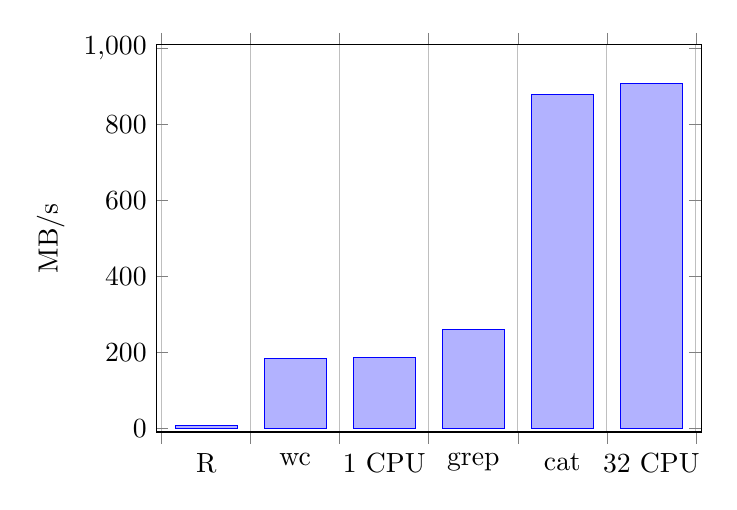
\begin{tikzpicture}
\begin{axis}[
	ylabel=MB/s,
  ymin=0, ymax=1000,
	enlargelimits=0.01,
	ybar interval=0.7,
  symbolic x coords={R, wc, 1 CPU, grep, cat, 32 CPU, end},
  width=8.5cm, height=6.5cm,
]
\addplot coordinates {(R,6.0) (wc,182.6) (1 CPU,186.6) (grep,261) (cat,878) (32 CPU,908) (end,0) };
% \addplot coordinates {(R,6.0) (wc,182.6) (CPU1,186.6) (grep,261) (wc -l,852) (cat,878) (Run 372,908) (Run 1,1029) (end,0) };

% \legend{MB/s}

\end{axis}
\end{tikzpicture}
\end{center}

\caption{Throughput comparisons of Icicle (1 CPU and 32 CPU) against existing R code and standard Unix utilities; higher is faster.}
\label{icicle:fig:bench:other}
\end{figure}



The graph in \cref{icicle:fig:bench:other} shows the throughput in megabytes per second.
We compared the throughput of several programs over the same dataset:
\begin{itemize}
\item our original R implementation (R);
\item Icicle running single-threaded (1 CPU);
\item Icicle running on multiple processors (32 CPU);
\item finding empty lines with @grep "^$"@ over the same data;
\item counting characters, words and lines with @wc@;
\item reading and throwing away the results with @cat > /dev/null@.
\end{itemize}

We ran all the Unix utilities with unicode decoding disabled using @LANG=C LC_COLLATE@ for maximum performance. The input data does not contain unicode characters. 
We used an Amazon EC2 @c3.8xlarge@ with 32 CPUs, 60GB of RAM, and striped, RAIDed SSD storage. The fused Icicle version significantly outperformed the R version of the queries, and the single-threaded version was on par with @wc@, while only a little slower than @grep@. This is despite the fact that the Icicle queries perform more computational work than @wc@ and @grep@. By using multiple processors, we were able to scale up to perform as well as @cat@, approaching the disk speed.
The memory usage of Icicle starts at around 200MB of RAM for a single thread, but as more threads are added approaches 15MB per thread.
The memory usage is constant in the input size and depends on the number of queries.
The R code is single threaded and would require at least 150 processors to reach similar speeds, assuming perfect scaling.
% These results give us confidence that our distributed implementation will be fast as well as scalable~\cite{mcsherry2015scalability}.


% The R code requires an @i2.8xlarge@ with 244GB of memory, but we were unable to perform our other benchmarks on such a large machine.
% \BEN{I wouldn't worry about stating this. You can't give out your R code so no one will test it themselves, and if even if you could run it on the smaller machine it wouldn't be faster}

% We were able to achieve such good results by generating parsing code specialised to the schema, and using data-only flattening~\cite{bergstrom2013data} as an efficient representation of structures such as arrays of sum types and tuples.
% \BEN{This isn't part of the contribution of this paper, so there's no real reason to discuss it}.

% By using a query plan that is close to a functional language, we are able to apply many standard optimisations such as common subexpression elimination and dead code removal.
% \BEN{We already said this before}. 



%!TEX root = ../Main.tex

\begin{figure}

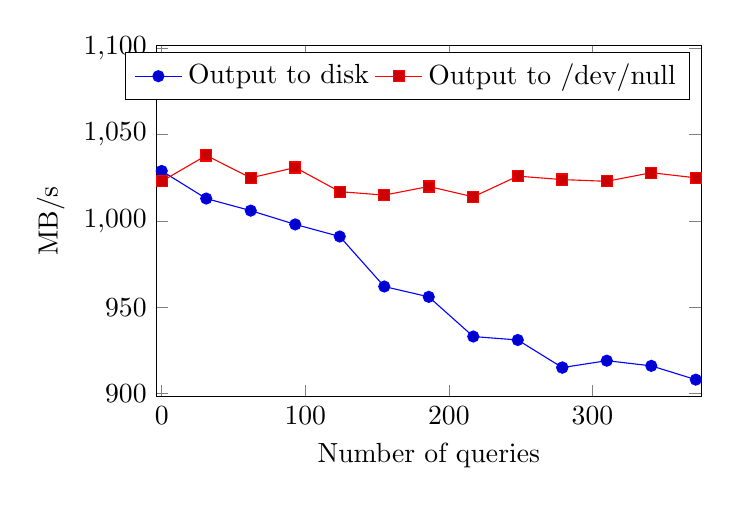
\begin{tikzpicture}
\begin{axis}[
	x tick label style={/pgf/number format/1000 sep=},
	ylabel=MB/s,
  ymin=900, ymax=1100,
%  xmax=372,
  xlabel=Number of queries,
	enlargelimits=0.01,
	legend style={legend columns=-1},
  width=8.5cm, height=6.05cm,
%	legend style={at={(0.5,-0.1)},anchor=north,legend columns=-1},
%	ybar interval=0.7,
]

% bench/raw.txt
% Running with fewer queries
% \addplot coordinates {(0,1025.5) (1,1029.6) (48,978) (96,941) (144,943) (192,936) (240,904) (276,895.5) (324,881) (372,846.2) };

% bench/raw.txt
% Running with fewer queries, better distribution
% \addplot coordinates { (0,1029) (31,1013) (62,1006) (93,998) (124,991) (155,941) (186,956) (217,933) (248,931) (279,915) (279,915) (310,919) (341,916) (372,908) };

%% APPLY LOPASS
\addplot coordinates { (0,1029) (31,1013) (62,1006) (93,998) (124,991) (155,962) (186,956) (217,933) (248,931) (279,915) (279,915) (310,919) (341,916) (372,908) };


% Fusion, no output
% \addplot coordinates { (0,1001) (31,1038) (62,1025) (93,1031) (124,1006) (155,1015) (186,1020) (217,997) (248,1026) (279,1024) (310,1009) (341,1038) (372,1025) };

%% APPLY LOPASS
\addplot coordinates { (0,1023) (31,1038) (62,1025) (93,1031) (124,1017) (155,1015) (186,1020) (217,1014) (248,1026) (279,1024) (310,1023) (341,1028) (372,1025) };

% No fusion, no output
% \addplot coordinates { (0,987) (31,1037) (62,1024) (93,1002) (124,1037) (155,1024) (186,1004) (217,1040) (248,1023) (279,998) (310,1018) (341,1013) (372,1003) };

\legend{Output to disk, Output to /dev/null};

\end{axis}
\end{tikzpicture}


\caption{Decrease in read throughput as queries are added, comparing writing the output to disk and writing to /dev/null.}
\label{icicle:fig:bench:queries}
\end{figure}


% \begin{figure}
% \begin{tikzpicture}
% \begin{axis}[
% 	x tick label style={/pgf/number format/1000 sep=},
% 	ylabel=MB/s,
%   ymin=0, ymax=1200,
%   xlabel=Number of threads,
% 	enlargelimits=0.01,
% 	legend style={legend columns=-1},
% ]
% \addplot coordinates { (1,163) (2,335) (3,442) (4,532) (5,578) (6,615) (7,633) (8,628) (9,631) (10,626) (11,637) (12,643) (13,658) (14,795) (15,781) (16,798) (17,840) (18,864) (19,862) (20,867) (21,847) (22,877) (23,876) (24,884) (25,862) };
% \end{axis}
% \end{tikzpicture}
% \caption{Scaling as threads are added}
% \label{icicle:fig:bench:scaling}
% \end{figure}




\Cref{icicle:fig:bench:queries} shows how the total read throughput scales as the number of fused queries is increased.
For each number of queries, we ran two versions of the fused result: one version that wrote the output to disk, and the other that piped the result to @/dev/null@.
The graph shows the throughput of the disk version decreasing roughly linearly in the number of queries, while the version ignoring the output remains constant.
This suggests that we are IO bound on the write side, as we write the query results for each of the million end-users.
The time spent evaluating the queries themselves is small relative to our current IO load.


To achieve these benchmark results, we perform several low-level optimisations on the fused imperative code, in addition to the high-level fusion and common subexpression elimination optimisations already discussed.
One of the most important optimisations is generating specialised parsing and output code.
Many of our data sets are stored as text files containing JSON values.
The format for these JSON values is dictated by the type of each query's input table.
For each fused set of queries, we generate C code that parses the input table, computes the result of the query, and writes the result to an output file.
The generated parsing and output code is specific to the input and output types, as opposed to generic JSON parsing code that must dynamically allocate records with statically unknown fields.



% This suggests that the output code is the bottleneck, which is unsurprising given the output format is text-based PSV.
% computing the queries appears constant as hundreds of queries are added, which suggests that many more queries can be handled if a better output format is used.
% \BEN{I don't understand this, surely the program would produce the PSV even if it was just sent to /dev/null?}
